\section{Queues}

Until now, we saw that the use of global variables made it possible to exchange information between two tasks. This method however presents some disadvantages among which the fact that a task is not automatically informed of a change of the variable. It is thus necessary that the task checks it periodically (polling) or that it announces any change via a mutex or semaphore.

To make this exchange easier, \rtos~implements another protocol: \textbf{queues}.

A task or an ISR can deposit a message in a queues. In a similar way, one or more tasks can receive a message in this queue.

Note: when we speak about ``message" under \rtos, it actually acts as any kind of structure copied in a reserved memory. The type of structure must obviously be known by the transmitting task as well as the receiving task(s).

% \begin{center}
%     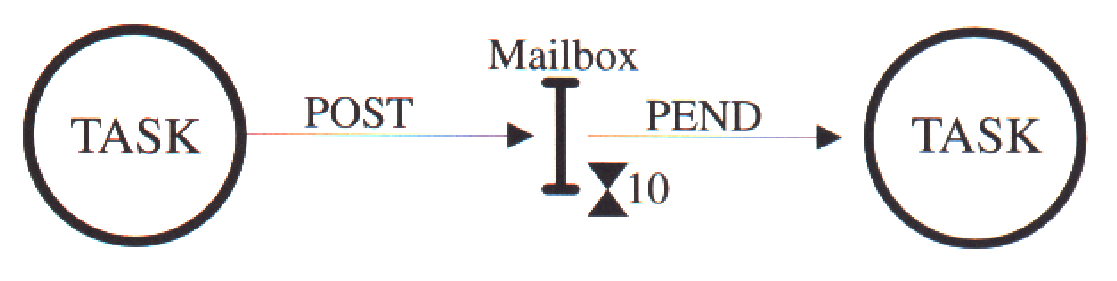
\includegraphics[width=12cm]{mailbox.png}
% \end{center}

If a task wishes to receive a message coming from a queue, it is suspended until the arrival of the message, or during a lapse of time defined by the application. Each queues is thus associated to a waiting list containing these suspended tasks. When the message is posted, it's the highest priority waiting task that receives the message\footnote{for more details see
\url{https://www.freertos.org/Embedded-RTOS-Queues.html}}.

Open the project \kw{keyboard}.
 
This project contains two tasks :
\begin{itemize}
    \item \kw{keyboardTask} is the task which manages the keyboard: if a new key is pressed, the \kw{key} variable contains the ASCII code of this key. The task is reactivated every 50ms to detect the actions of the user. It makes use of the \kw{KB\_Scan()} API of the block \kw{keyboard\_4x3}. This block was custom made for these labs and is part of the \kw{extensionBoardLib} library. Make sure your project includes the library by right clicking on the project tab > Dependencies and verify that the extensionBoardLib is checked. Also, make sure that the keyboard is correctly connected to the extension board, see Appendix~\ref{ap:kb}.
    \item \kw{lcdTask} displays a character on the LCD screen. Read the datasheet of the \kw{Character LCD} block to understand how it interact with the LCD screen.
\end{itemize}

\E{
    Create a queue allowing to transmit the characters pressed on the keyboard to the task displaying the characters on the screen. The queue should only contain one message.
}{}
%\marginpar{OK add caption and refr to listing} done

